\subsection{Task Description}
The {\href{http://www.languageworkbenches.net/images/5/53/Ql.pdf}{LWC13 task}}
is to implement a DSL for questionnaires (Questionnaire Language, QL), which
basically allows the definition of forms with questions.

We assume that you have read the LWC13 assigment document carefully before
continuing reading this document.


\subsection{Technology Stack}
\label{subsec:technologyStack}
This tutorial expects that you are somehow familiar with Java and Eclipse and
have heard about \url{EMF} and how it works in general before. We start almost at the
beginning, but not quite :-) 

\subsubsection*{Grammar Definition}
We will use Xtext 2.4.0, which is at the moment of writing the latest official
release.
Xtext 2.5 is in preparation and will be released with Eclipse Kepler in June
2013\footnote{\url{http://wiki.eclipse.org/Kepler/Simultaneous_Release_Plan}}.
The solution approach described here would work also with any version
of Xtext >= 2.0, but the API might differ slightly, so there is no guarantee
that each codeline printed here would work exactly with all versions. For better
reproduction it is highly recommended to use the versions mentioned above.

\subsubsection*{Code Generator}
For Code Generation we will use the language Xtend, which itself is based on
Xtext. Xtend makes use of a common expression language shipped with Xtext called
Xbase. The languages developed here will also be based on Xbase, but more on
this later.

\subsubsection*{Questionnaire Application}
The developed code generator will generate
JavaServer Faces 2.1 (JSF)\footnote{\url{http://www.javaserverfaces.org/}} pages
in XHTML file format. JSF is part of the Java Enterprise Edition (Java EE). It
is useful to have a basic understanding of how web applications work even if JSF provides a nice level 
of abstraction. The JSF reference implementation from 
Oracle Mojarra 2.1.6\footnote{\url{http://javaserverfaces.java.net/}} is able to run 
within the well known Servlet container Apache Tomcat(
v7.0)\footnote{\url{http://tomcat.apache.org/}}. In order to not reload the
whole page whenever some content needs to be updated (e.g. optional questions
need to be displayed depending on other questions' answers) we will use AJAX.
The following screenshot shows the resulting application:

\begin{center}
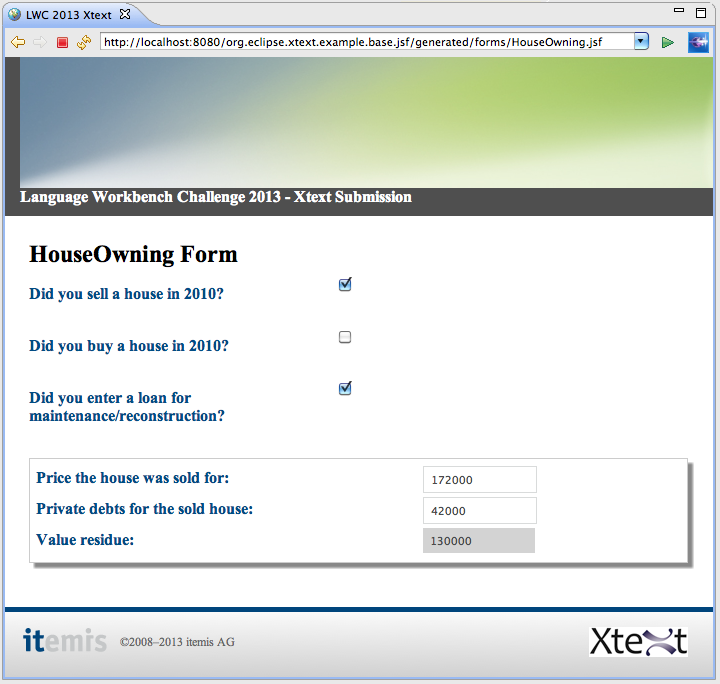
\includegraphics[width=15cm]{./images/chapter02/questionnaireApplication.png}
\end{center}

